% !TeX root = ../presentation.tex

\section{Potenziale und Ziele}

\begin{frame}{Vertrauen}
    \textbf{Warum kein Vertrauen?}
    \begin{itemize}
        \item Angst vor Datenmissbrauch oder unberechtigter Weitergabe~\cite{mollerIndustrialDataEcosystems2024}
    \end{itemize}

    \pause
    \textbf{Was würde helfen?}
    \begin{itemize}
        \item Verwaltung von Daten durch Nutzende unabhängig von Anwendungen
        \item Daten im Besitz der Nutzenden
        \item Kontrolle über Daten und Zugang

        \pause
        \item[$\Rightarrow$] Datensouveränität \& Datenschutz
    \end{itemize}
\end{frame}

\begin{frame}{Vertrauen II}
    \begin{columns}
        \begin{column}{0.6\textwidth}
            \textbf{Wem kann ich vertrauen?\\Ist das wirklich dieser Akteur?}
            \begin{itemize}
                \item[$\to$] Authentifizierungsverfahren
                \item[$\to$] Vertrauen in geteilte Daten
                
                % jemand will Studie mit falschen Daten verfälschen, Medikament was nicht wirkt
        
                \item[$\Rightarrow$]<2-> über Vertrauen in andere Akteure
                \item[$\Rightarrow$]<2-> ad"=hoc Data Sharing möglich
            \end{itemize}
        \end{column}

        \begin{column}{0.4\textwidth}
            \begin{figure}
                \centering
                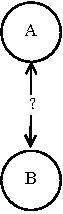
\includegraphics[height=5cm]{./assets/trust_question.drawio.pdf}
                \caption{Symbolbild Vertrauen}
            \end{figure}
        \end{column}
    \end{columns}
\end{frame}

\begin{frame}{Vertrauen III}
    \textbf{Einhaltung gesetzlicher Vorgaben}
    \begin{itemize}
        \item technische Maßnahmen notwendig

        \pause
        \item physische und logische Trennung von Datenspeichern je nach Kontext
        \begin{itemize}
            \item bspw. Medizin"= getrennt von Bewerbungsdaten
        \end{itemize}

        \pause
        \item[$\Rightarrow$] Dezentralisierung
        \item[$\Rightarrow$] Interoperabilität auf Daten"= statt Anwendungsebene
    \end{itemize}
\end{frame}


\begin{frame}{Aktualität und Verfügbarkeit von Daten}
    \textbf{Warum veraltet und schlecht verfügbar?}
    \begin{itemize}
        \item Angst vor Datenmissbrauch und unberechtigter Weitergabe $\to$ mangelndes Vertrauen

        \pause
        \item[$\to$] Datensouveränität und Datenschutz
        \item[$\to$] höhere Wahrscheinlichkeit zur Speicherung von mehr und diverseren Daten

        \pause
        % Verfügbarkeit?
        \item[$\to$] Interoperabilität, offene Standards

        \pause
        \item[$\Rightarrow$] Aktualität und Verfügbarkeit von Daten
    \end{itemize}
\end{frame}


\begin{frame}{Kosten, Effizienz und Geschwindigkeit}
    \textbf{Was ist so teuer?}
    \begin{itemize}
        \item aufwendige Integrationen durch unterschiedliche Datenstrukturen
        \item wiederholte Schritte, bspw. Implementierung von Standardfunktionalitäten
    \end{itemize}

    \pause
    \textbf{Was würde helfen?}
    \begin{itemize}
        \item Auslagerung von Standardfunktionalitäten, Wiederverwendbarkeit, Interoperabilität
        \item[$\Rightarrow$] Automatisierung $\Rightarrow$ Kostensenkung, schnelle Prozesse
        \item[$\Rightarrow$] ad-hoc Zusammenschaltung von Geschäftsprozessen
    \end{itemize}
\end{frame}


\begin{frame}{Zugänglichkeit}
    \begin{itemize}
        % wenn oben erfüllt, dann können wir ... entgegenwirken
        \item[?] hohe Kosten und Aufwand
        \pause
        \begin{itemize}
            \item Automatisierung $\to$ niedrigere Kosten und Aufwand
        \end{itemize}

        \pause
        \item[?] wenig verfügbare Daten, proprietäre Datenformate
        \pause
        \begin{itemize}
            \item breitere Verfügbarkeit von Daten, Interoperabilität, offene Standards
        \end{itemize}
    \end{itemize}

    \pause
    \begin{itemize}
        \item[$\Rightarrow$] niedrigere Einstiegsbarrieren
        \item[$\Rightarrow$] Zugänglichkeit $\Rightarrow$ Wettbewerb, Innovation
    \end{itemize}
\end{frame}


\begin{frame}{Wie erreichen wir das?}
    \fbox{Datensouveränität\strut}
    \fbox{Dezentralisierung\strut}
    \fbox{Interoperabilität\strut}
    
    \fbox{Verfügbarkeit \& Aktualität\strut}
    \fbox{Automatisierung\strut}
    \fbox{ad-hoc Authentifizierung\strut}

    \vspace{1em}

    \begin{itemize}
        \large
        \item[$\Rightarrow$] Kooperation verschiedener Akteure in einem vertrauenswürdigen, offenen, interoperablen System für Data Sharing
    \end{itemize}

    % hier setzt Konzept Data Spaces an
    % ermöglicht multilaterales, sicheres Data Sharing
    % Garantie von Datensouveränität
\end{frame}
